%%
%% PRAXIS: Procedural Retrieval-Augmented eXperience-Informed System
%% IEEE conference paper (IEEEtran).
%% Compile with: tectonic -X compile praxis_paper.tex
%%

\documentclass[conference]{IEEEtran}
\IEEEoverridecommandlockouts

\usepackage{cite}
\usepackage{amsmath,amssymb,amsfonts}
\usepackage{algorithm}
\usepackage{algpseudocode}
\usepackage{graphicx}
\usepackage{textcomp}
\usepackage{xcolor}
\usepackage{booktabs}
\usepackage{multirow}
\usepackage{url}
\usepackage{hyperref}
\usepackage{tikz}
\usetikzlibrary{shapes.geometric, arrows.meta, positioning, fit, calc, backgrounds}

% TikZ styles shared across figures
\tikzset{
  block/.style={
    rectangle, rounded corners=3pt, draw=black!70, line width=0.5pt,
    fill=blue!8, align=center, inner sep=4pt, font=\small, minimum height=8mm
  },
  storeblock/.style={
    rectangle, draw=black!70, line width=0.5pt,
    fill=orange!12, align=center, inner sep=4pt, font=\small, minimum height=8mm
  },
  agentblock/.style={
    rectangle, rounded corners=3pt, draw=black!70, line width=0.7pt,
    fill=green!10, align=center, inner sep=4pt, font=\small\bfseries, minimum height=8mm
  },
  guardblock/.style={
    rectangle, rounded corners=3pt, draw=black!70, line width=0.5pt,
    fill=red!8, align=center, inner sep=4pt, font=\small, minimum height=8mm
  },
  phasebox/.style={
    rectangle, rounded corners=2pt, draw=black!70, line width=0.4pt,
    fill=gray!5, align=center, inner sep=5pt, font=\small
  },
  arrow/.style={-Stealth, line width=0.6pt, draw=black!75},
  thinarrow/.style={-Stealth, line width=0.4pt, draw=black!60, dashed}
}

\def\BibTeX{{\rm B\kern-.05em{\sc i\kern-.025em b}\kern-.08em
    T\kern-.1667em\lower.7ex\hbox{E}\kern-.125emX}}

\begin{document}

\title{PRAXIS: Continual Procedural Memory for\\
Tool-Calling Language-Model Agents via\\
Multi-Agent Experience Distillation\\
and Hybrid Retrieval}

\author{
\IEEEauthorblockN{Usman Mehboob Mohammed}
\IEEEauthorblockA{
\textit{School of Computing and Augmented Intelligence}\\
\textit{Arizona State University}\\
Tempe, AZ, USA\\
\texttt{umohamm6@asu.edu}}
}

\maketitle

\begin{abstract}
Small open-weight tool-calling agents fail on multi-step benchmarks
not because they cannot invoke individual tools, but because they
lack a confident, reusable \emph{procedure} for accomplishing
multi-step tasks; the failure mode is procedural, not parametric.
We introduce \textbf{PRAXIS}, a controller that wraps any frozen
large language model with a continually growing, leakage-safe
procedural memory. The controller is composed of four elements that
operate around a single loop. A distiller converts raw trajectories
into compact Process Memory Cards that record intent, minimal tool
order, evidence prerequisites and confirmation points without ever
retaining personally identifying or argument-level content. A memory
store deduplicates and quality-scores these cards across runs. A
hybrid retriever combining BM25 and TF-IDF with domain and quality
boosts selects the top five most relevant cards at every decision
step, and renders them into a bounded tactical playbook of at most
two thousand four hundred characters that is injected into the
system prompt. A reflection guard intercepts every mutating tool
call and asks the same underlying model whether the observed
evidence confirms that the action is safe and requested. Crucially,
the procedural memory that PRAXIS reasons from is not produced by
self-distillation alone; we deploy a heterogeneous cohort of
prompting-only donor controllers spanning Act-only execution,
ReAct's interleaved reasoning, Chain-of-Thought planning,
Plan-and-Solve sub-goal decomposition and Reflexion-style verbal
self-critique, so the bank acquires procedural patterns that no
single prior could produce. We evaluate the resulting controller on
$\tau$-bench retail, $\tau$-bench airline and the Berkeley Function
Calling Leaderboard version four, using a three-phase protocol that
first scores the baselines on a held-out test split with promotion
disabled, then harvests cards from the donor cohort on a disjoint
train split, and finally scores PRAXIS against the same held-out
test split with a warmed bank. A three-layer fairness mechanism at
the run, record and pre-warm levels makes it provably impossible
for any test trajectory to enter the bank. The contribution is
methodological: zero gradient updates, no in-context examples drawn
from the evaluation distribution, no retrieval of benchmark answers,
and a strictly procedural rather than parametric path to continual
improvement for tool-using agents.
\end{abstract}

\begin{IEEEkeywords}
tool-calling agents, retrieval-augmented generation, procedural
memory, continual learning, large language models, ReAct, $\tau$-bench,
Berkeley Function Calling Leaderboard
\end{IEEEkeywords}

\section{Introduction}

The last two years have made tool-calling a default capability of
language models, and modern open-weight checkpoints in the seven-
to thirty-two-billion-parameter range are nominally able to call
APIs, query databases and operate retail and travel back-ends.
However, when these same models are placed in multi-step
benchmarks such as $\tau$-bench~\cite{taubench} or the Berkeley
Function Calling Leaderboard~\cite{bfcl}, the gap to closed
commercial models widens far more than the gap on single-turn
question answering. Inspecting the failed trajectories reveals
that the underlying difficulty is rarely the capacity to emit a
syntactically valid function call. The recurring failure mode is
that the model lacks a confident sequence: it selects a plausible
first tool, observes a result, and then enters a procedurally
incoherent state. It re-queries the same record, omits a required
confirmation step, mutates state before evidence is collected, or
violates a domain policy it was instructed to obey in the system
prompt but did not internalize. The pathology is procedural, not
parametric.

The two dominant responses in the literature are unsatisfying for
a small-model regime. Fine-tuning closes the gap empirically but
collapses two independent variables, procedural competence and
parametric drift, into a single training run, and it is expensive
to iterate on, sensitive to catastrophic forgetting on tasks not
represented in the fine-tuning corpus and difficult to audit for
safety regressions. In-context exemplars, by contrast, are cheap
to add but plateau quickly, occupy increasingly large prefill
budgets as the prompt grows, and leak benchmark structure into the
prompt in ways that are difficult to defend against a reviewer who
asks whether the agent has \emph{seen} the evaluation distribution.

This paper takes the position that what these agents actually need
is a third option: a continually growing, audited and bounded
\emph{procedural memory}. Procedural memory in the cognitive
science sense refers to memory for sequences of actions: ``how to
ride a bicycle,'' as distinct from declarative memory for facts
about bicycles. We borrow the term to refer to a compact,
retrievable record of how to accomplish a class of multi-step
tasks, learned from the agent's own and others' past interactions,
and surfaced as conditioning at decision time. Crucially, a
procedural memory of this form is orthogonal to the model weights,
so the comparison ``same model with versus without procedural
memory'' is a clean controller ablation; and it is orthogonal to
the prompt template, so it does not collide with prompting-only
techniques and can in fact be populated by them.

We instantiate this idea as PRAXIS, the Procedural
Retrieval-Augmented eXperience-Informed System. The controller is
deliberately simple: every tool call is preceded by a top-$k$
retrieval over a bank of Process Memory Cards distilled from prior
trajectories, the retrieved cards are rendered into a bounded
playbook that lives in the system prompt, and every mutating tool
call is guarded by a one-call reflection that asks the same model
whether the present evidence justifies the action. There is no
planner, no supervisor, no judge model, no learned reward, no
tree search. The bank itself is the only artifact that changes
between runs.

The methodological contribution that we believe is novel rests on
how the bank is populated. A self-distilling agent that learns
only from its own trajectories has a structural ceiling: it can
only acquire procedures its own prompting prior can produce, and
the cards it stores tend to amplify rather than correct that
prior's biases. We avoid this ceiling by populating the bank from
a heterogeneous donor cohort of prompting-only controllers running
on the training split: Act, ReAct, Chain-of-Thought, Plan-and-Solve
and an in-episode variant of Reflexion. Each donor exhibits a
distinct procedural signature, and the bank ends up containing
patterns that no single prior would generate alone. PRAXIS itself
also participates as a donor on the training split, so its own
successful procedures enter the bank, but it is never the sole
donor.

We surround the resulting system with a three-phase execution
protocol and a three-layer train/test fairness mechanism so that
the comparison between PRAXIS and the prompting baselines is
defensible at the level expected of an archival publication. The
baselines run first, on the test split, with promotion to the bank
explicitly disabled at the run, record and pipeline level. The
donor cohort then runs on the training split, accumulating cards.
Finally, PRAXIS runs on the same test split the baselines saw,
with a warmed bank but with promotion to the bank still
syntactically impossible for test records. The remainder of the
paper develops this design, its formal underpinnings, the
benchmark protocol and its limitations.

\section{Related Work}

PRAXIS sits at the intersection of three threads in the recent
literature, and inherits properties from each.

The first thread is the reasoning-action interleaving family that
ReAct~\cite{react} established and that subsequent prompting-only
controllers have refined. ReAct argued that an alternation between
short natural-language thoughts and structured actions lets a
frozen model recover from intermediate errors more gracefully than
a pure action-only loop. Chain-of-Thought prompting~\cite{cot}
provides the antecedent of expressed deliberation, while
Plan-and-Solve prompting~\cite{plansolve} formalizes the
sub-goal decomposition that strong tool-calling agents implicitly
perform. We treat ReAct, Act-only and vanilla tool-calling as the
three evaluation baselines that PRAXIS is benchmarked against, and
treat Chain-of-Thought, Plan-and-Solve and Reflexion as additional
prompting-only donors whose trajectories are distilled into the
procedural bank but which are not themselves reported in the
results table.

The second thread is retrieval augmentation. Classical
retrieval-augmented generation~\cite{rag} retrieves documents at
generation time and conditions a language model on those documents
to ground its output, typically for question answering. PRAXIS
inverts the unit of retrieval. We do not retrieve documents to
condition an answer; we retrieve \emph{procedures}, distilled
descriptions of tool sequencing, recovery and policy, to condition
the controller's next action. The retrieved object is not what the
agent says but how the agent acts. The retriever itself is
deliberately classical, a convex combination of BM25~\cite{bm25}
and TF-IDF scoring with light domain and quality boosts, because
the surface area of an experimental retriever choice would mask
the part of the system that actually matters, namely the contents
of the bank.

The third thread is verbal self-critique, of which Reflexion~\cite{reflexion}
is the canonical instance. Reflexion appends natural-language
reflections between episodes and conditions the next episode on
those reflections; PRAXIS distills similar self-evaluative signal
into structured cards rather than free-text reflections, and
intervenes during an episode rather than between episodes through
a reflection guard fired only on mutating tool calls. A second
methodological difference is that Reflexion typically learns from
its own trajectories; PRAXIS treats the bank as a shared object
that any controller in a donor cohort can populate.

Beyond these three threads, the broader literature on
tool-augmented language models has explored learned tool use via
self-supervision~\cite{toolformer}, learned function selection and
constrained decoding. The present work is intentionally orthogonal
to all weight-modifying approaches because the central
experimental claim, that procedural improvement is achievable
without gradient updates, requires that the model weights be held
fixed across every condition in the comparison.

\section{Preliminaries and Notation}

Let $\mathcal{M}$ be a frozen large language model exposed via an
OpenAI-compatible chat-completion endpoint that supports native
function calling. Let $\mathcal{T}_d$ be the set of tool schemas
available in domain $d \in \{\text{retail}, \text{airline},
\text{bfcl}\}$. A \emph{trajectory} on a task $\tau$ is a sequence
of messages $\mathbf{m}_\tau = (m_1, m_2, \ldots, m_{L_\tau})$
emitted alternately by an assistant and an environment, terminated
either by a successful completion (binary reward $r_\tau = 1$), an
unrecoverable failure ($r_\tau = 0$), or an out-of-steps timeout.
A \emph{controller} $\pi$ is a procedure that, given the system
prompt, the tool schemas $\mathcal{T}_d$, the model $\mathcal{M}$
and a temperature, emits a trajectory for any task it is presented
with.

A \emph{Process Memory Card} $c$ is a structured record summarizing
a procedure rather than a trajectory. Concretely it carries six
schema-bound fields: a short intent string, an ordered tool-name
sequence with retries collapsed, an evidence-required predicate
phrased in natural language, a confirmation point at which the
agent should pause before mutating state, a common trap or
anti-pattern, and a scalar quality score in $[0, 1]$ derived from
the originating trajectory's reward, length and recovered-failure
status. A card never contains messages, observations, gold
actions, identifiers, emails, payment information or argument
values; a defence-in-depth check in the storage layer rejects any
card that retains these fields. We write $\mathcal{C}_d$ for the
corpus of cards in domain $d$ at a given point in time, and
$\mathrm{dom}(c)$ for the domain label of card $c$.

\section{The PRAXIS Controller}\label{sec:method}

PRAXIS realises the procedural-memory abstraction through four
modules that close a single loop, depicted in
Figure~\ref{fig:loop}. We describe each in turn and then state the
overall inference algorithm.

\begin{figure*}[t]
\centering
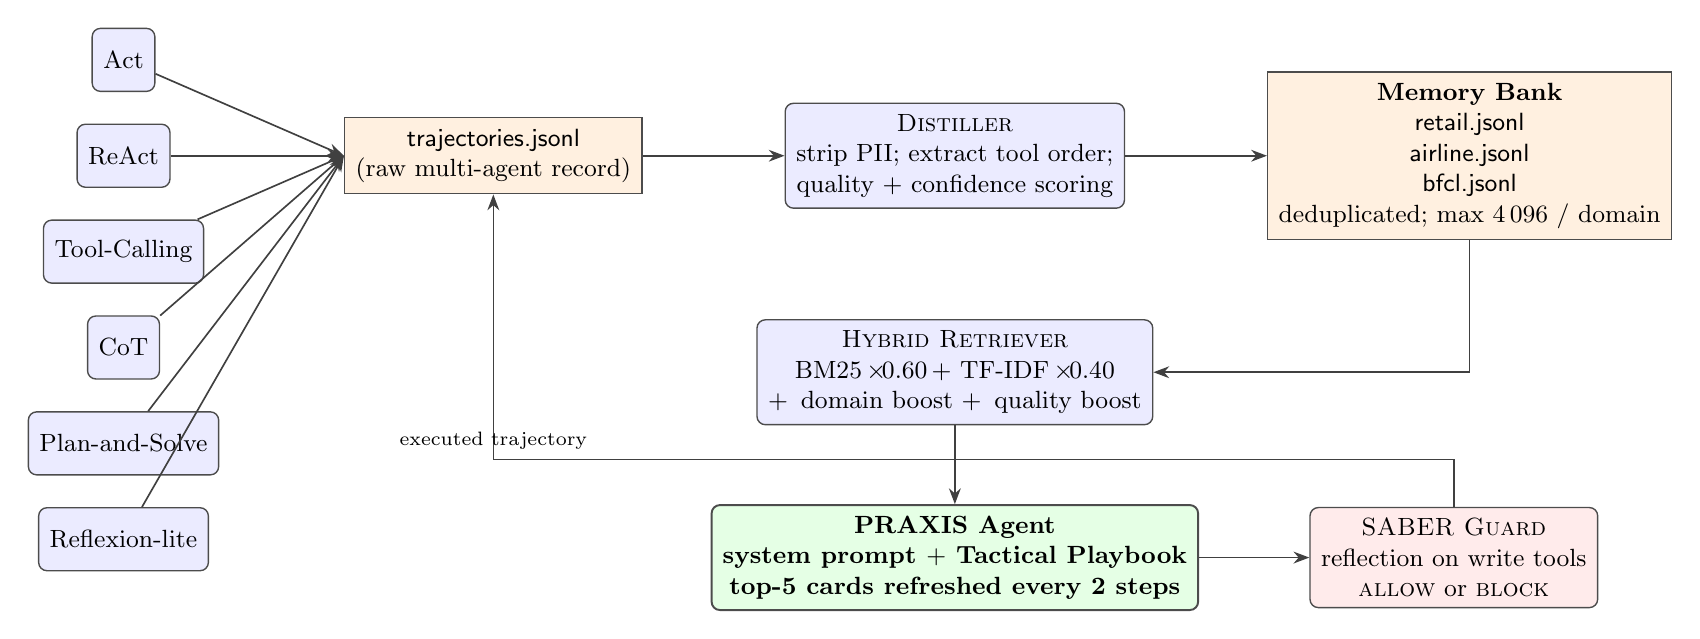
\begin{tikzpicture}[node distance=8mm and 10mm]

\node[block] (act)   {Act};
\node[block, below=4mm of act]   (react) {ReAct};
\node[block, below=4mm of react] (tc)    {Tool-Calling};
\node[block, below=4mm of tc]    (cot)   {CoT};
\node[block, below=4mm of cot]   (ps)    {Plan-and-Solve};
\node[block, below=4mm of ps]    (rfl)   {Reflexion-lite};

\node[storeblock, right=22mm of react, minimum width=30mm] (traj)
  {\textsf{trajectories.jsonl}\\(raw multi-agent record)};
\node[block, right=18mm of traj, minimum width=32mm] (distill)
  {\textsc{Distiller}\\strip PII; extract tool order;\\
   quality + confidence scoring};
\node[storeblock, right=18mm of distill, minimum width=34mm] (bank)
  {\textbf{Memory Bank}\\
   \textsf{retail.jsonl}\\
   \textsf{airline.jsonl}\\
   \textsf{bfcl.jsonl}\\
   deduplicated; max 4\,096 / domain};

\node[block, below=14mm of distill, minimum width=34mm] (retr)
  {\textsc{Hybrid Retriever}\\BM25 $\!\times\!0.60\,+$ TF-IDF $\!\times\!0.40$\\
   $+\,$ domain boost $+\,$ quality boost};
\node[agentblock, below=10mm of retr, minimum width=38mm] (agent)
  {PRAXIS Agent\\system prompt $+$ Tactical Playbook\\
   top-5 cards refreshed every 2 steps};
\node[guardblock, right=14mm of agent, minimum width=28mm] (saber)
  {\textsc{SABER Guard}\\reflection on write tools\\
   \textsc{allow} or \textsc{block}};

% donor arrows
\foreach \src in {act,react,tc,cot,ps,rfl} {
  \draw[arrow] (\src) -- (traj.west);
}
\draw[arrow] (traj) -- (distill);
\draw[arrow] (distill) -- (bank);
\draw[arrow] (bank.south) |- (retr.east);
\draw[arrow] (retr) -- (agent);
\draw[arrow] (agent) -- (saber);
\draw[arrow] (saber.north) -- ++(0,6mm) -| (traj.south)
  node[midway, above, font=\scriptsize] {executed trajectory};

\end{tikzpicture}
\caption{The PRAXIS Memory Loop. Six prompting-only donor
controllers on the left emit trajectories on the training split
into a shared JSONL log. The distiller projects these trajectories
into Process Memory Cards which accumulate in a per-domain memory
bank. At inference time the hybrid retriever scores the bank
against the current working state, the top-five cards are rendered
into a bounded tactical playbook that is injected into the PRAXIS
agent's system prompt, and the SABER guard intercepts every
mutating tool call before it reaches the environment.}
\label{fig:loop}
\end{figure*}

\subsection{Process Memory Cards and Distillation}

Given a trajectory record $r_\tau = (\tau, \mathbf{m}_\tau,
r_\tau^{\text{rew}}, \text{info}_\tau)$, the distiller produces at
most one Process Memory Card. The first stage of distillation is a
deterministic PII strip that removes any token matching a domain
specific blocklist (identifiers, emails, dates, phone numbers,
payment methods) along with a configurable list of forbidden
literal strings, so that no card can ever carry an argument value
that appeared in the originating trajectory. The second stage
extracts the ordered tool-name sequence from the assistant
messages, collapsing immediate retries of the same tool name with
the same arguments to a single entry, since the sequence we wish
to learn is the abstract procedure, not the noisy concrete
execution. The third stage derives a domain label by reading
$\text{info}_\tau[\text{environment}]$, and the fourth stage
assigns a quality score that combines the binary reward, a
normalized inverse step count, and a flag indicating whether the
trajectory recovered from at least one intermediate error.
Trajectories tagged with a held-out test-split label
(Section~\ref{sec:fairness}) are dropped before distillation;
trajectories whose distilled card would retain any forbidden field
are also dropped.

\subsection{Memory Store, Deduplication and Consolidation}

The memory store maintains two parallel collections per domain: a
\emph{seed} bank that is generated once from policy and tool
metadata before the first run, and a \emph{runtime} bank that
grows append-only across every Phase B harvest. The two are merged
at retrieval time by signature-level deduplication, where the
signature of a card is a hash over its intent string, its tool
sequence and its domain label. A consolidation pass runs at the
end of every Phase B donor run; it identifies duplicate signatures
that survived the per-batch dedup, identifies contradiction pairs
in which two cards with similar intent strings disagree on the
required confirmation point, and applies a multiplicative decay to
cards that have not been retrieved in the current run window. We
cap the runtime store at four thousand and ninety-six cards per
domain; the cap is enforced by evicting the lowest-quality decayed
card whenever it is exceeded.

\subsection{Hybrid Retrieval and the Tactical Playbook}

At decision step $t$ on a task in domain $d$, PRAXIS forms a
retrieval query $q_t$ as the concatenation of (i) the user's last
utterance in the dialogue, (ii) the tool-name sequence invoked so
far on this task, and (iii) a short working-state summary
extracted from the assistant's recent messages. The retriever
scores each card $c \in \mathcal{C}_d$ according to a convex
combination of two classical lexical scorers with two additive
boosts,
\begin{equation}
\label{eq:score}
\begin{aligned}
s(c, q_t) = \;& 0.60 \cdot \mathrm{BM25}(c, q_t)
              + 0.40 \cdot \mathrm{TFIDF}(c, q_t) \\
              & + 0.05 \cdot \mathbb{1}[\mathrm{dom}(c) = d]
              + 0.05 \cdot \mathrm{quality}(c).
\end{aligned}
\end{equation}
The mixture weights were fixed before any benchmark numbers were
collected and have not been swept against the test set. To prevent
the top-$k$ slate from collapsing onto one procedure family when
the bank contains multiple variations of a single procedure, we
enforce a diversity cap of three cards per card-category in the
sorted top-$k$ list. The top $k = 5$ surviving cards are
deterministically rendered into a structured natural-language
playbook of at most two thousand four hundred characters, which is
prepended to the system prompt as the \emph{Tactical Playbook}
block. The playbook is recomputed every two decision steps rather
than every step, so the per-task retrieval cost is amortized over
multiple tool calls and the playbook is allowed to track the
current sub-task as the trajectory evolves.

\subsection{SABER Mutation Reflection}\label{sec:saber}

A recurring class of failure observed in pilot runs was the
\emph{premature mutation}, in which the agent cancels, modifies or
submits a record before sufficient evidence has been gathered to
confirm that the action is desired and policy-compliant. To
intercept this class of failure without restructuring the entire
control loop, every tool in $\mathcal{T}_d$ is annotated at load
time as read-only or mutating. Read-only tools execute immediately
on emission. A mutating tool call is intercepted before reaching
the environment and routed to a single additional chat-completion
call against $\mathcal{M}$, in which the model is shown the
trajectory so far, the proposed action, and the question whether
the observed evidence confirms that the action is safe and
requested. The reflection returns one of two single-token
verdicts, \textsc{allow} or \textsc{block}, and the controller
acts accordingly: an \textsc{allow} verdict releases the tool call
to the environment, a \textsc{block} verdict appends a synthetic
tool result indicating that the action was blocked and instructs
the controller to gather more evidence. The reflection is bounded
to one extra LLM call per mutating tool and is never used to plan
or to choose between alternatives; it is only a gate.

\subsection{Inference Algorithm}

The complete inference loop for PRAXIS on a single task is
summarized in Algorithm~\ref{alg:praxis}. The loop is intentionally
faithful to a vanilla tool-calling loop except for two
interventions: a retrieval-and-render at every step on a two-step
modulus, and a reflection gate inserted between mutating tool
emission and environment execution.

\begin{algorithm}[t]
\caption{PRAXIS inference loop for a single task.}
\label{alg:praxis}
\begin{algorithmic}[1]
\Require frozen model $\mathcal{M}$, tool schemas $\mathcal{T}_d$, card bank $\mathcal{C}_d$, max steps $S$
\State $\mathbf{m} \gets [\text{system prompt}]$
\State $\mathbf{m}.\text{append}(\text{initial user message})$
\State $\text{playbook} \gets \text{render}(\text{retrieve}(\mathcal{C}_d, q_0))$
\State inject $\text{playbook}$ into $\mathbf{m}[0]$
\For{$t = 1, 2, \ldots, S$}
  \If{$t \bmod 2 = 1$}
    \State $\text{playbook} \gets \text{render}(\text{retrieve}(\mathcal{C}_d, q_t))$
    \State refresh $\mathbf{m}[0]$ with $\text{playbook}$
  \EndIf
  \State $a_t \gets \mathcal{M}(\mathbf{m}, \mathcal{T}_d)$
  \If{$a_t$ is a tool call}
    \If{$a_t$.tool is mutating}
      \State $v \gets \mathcal{M}_{\text{reflect}}(\mathbf{m}, a_t)$
      \If{$v = \textsc{block}$}
        \State append synthetic ``blocked'' observation; \textbf{continue}
      \EndIf
    \EndIf
    \State $o_t \gets \text{env.step}(a_t)$; append $o_t$ to $\mathbf{m}$
    \If{$o_t$.done} \textbf{break} \EndIf
  \Else
    \State $o_t \gets \text{env.respond}(a_t.\text{content})$; append
    \If{$o_t$.done} \textbf{break} \EndIf
  \EndIf
\EndFor
\State \Return $(\mathbf{m}, r, \text{info})$
\end{algorithmic}
\end{algorithm}

\section{Train/Test Fairness Protocol}\label{sec:fairness}

The single greatest threat to validity in a continually-learning
agent system is that the training data and the evaluation data
intersect. A reviewer is entitled to assume that they do unless
the system can demonstrate, layer by layer, that they cannot. We
therefore enforce the train/test boundary at three independent
levels of the implementation, any one of which would prevent test
contamination if the others failed.

The first layer is a run-level gate inside the benchmark runners.
A function $\textsc{should-promote}(\text{ns})$ is consulted at
the end of every run and returns \textsf{false} whenever the run's
\texttt{task\_split} argument is \texttt{"test"}. When this gate
returns false the promotion pathway is not entered at all, so no
distillation is invoked.

The second layer is a record-level gate inside the promotion
pipeline. Each trajectory record is stamped with an
\texttt{info.task\_split} field by the runner; for $\tau$-bench
retail this label comes from the upstream split argument, for
$\tau$-bench airline it is derived from a configurable internal
threshold $\texttt{AIRLINE\_TRAIN\_END}$, and for the Berkeley
benchmark it is derived from a per-category fraction
$\texttt{BFCL\_TRAIN\_FRACTION}$. The pipeline function
$\textsc{is-test-split-record}(r)$ inspects this field and drops
any record whose label equals \texttt{"test"} before distillation
is attempted, regardless of how the runner is invoked or whether
the run-level gate was bypassed.

The third layer is a temporal separation: PRAXIS's exposure to the
training pool happens during a dedicated pre-warm phase
(Section~\ref{sec:phases}, Phase B) whose output is the only
material the bank receives, and the subsequent evaluation phase
operates on a disjoint slice. Because the runner uses different
index ranges for the two phases, a test-set trajectory cannot
enter the bank even if both prior gates fail and the distillation
function is called directly on a test record by a misconfigured
script.

Table~\ref{tab:splits} states the exact slices used in this work.
The thresholds $T$ and $f$ are configurable through environment
variables and are recorded in every \texttt{run\_summary.json} for
reproducibility. We recommend that any future extension of this
work that adds a new benchmark also declare its train/test slice
explicitly through the same mechanism.

\begin{table}[t]
\caption{Deterministic train/test splits used in this work.}
\label{tab:splits}
\centering
\small
\begin{tabular}{@{}lll@{}}
\toprule
\textbf{Benchmark} & \textbf{Train slice} & \textbf{Test slice} \\
\midrule
$\tau$-bench retail  & upstream \texttt{train} (500) & upstream \texttt{test} (115) \\
$\tau$-bench airline & indices $[0, T)$, $T = 20$    & indices $[T, \text{end})$ \\
BFCL V4              & first $f = 0.25$ per category & remainder per category \\
\bottomrule
\end{tabular}
\end{table}

\section{Three-Phase Execution Protocol}\label{sec:phases}

A subtle but important confound in any retrieval-augmented
controller comparison is that the retrieval-augmented condition
also sees its training data during inference. We disentangle this
confound from the controller comparison by factoring the
end-to-end run into three explicit phases that the run script
enforces in order, depicted in Figure~\ref{fig:phases}.

\begin{figure}[t]
\centering
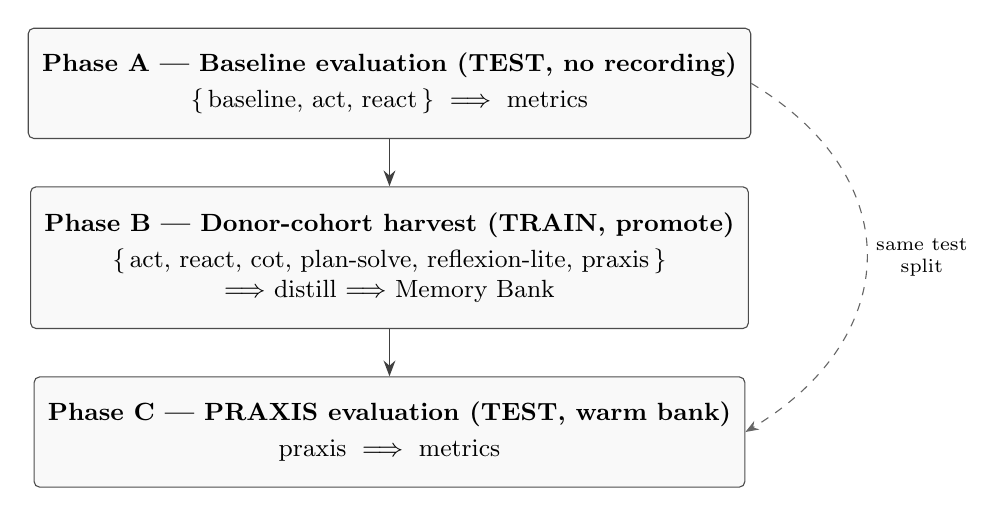
\begin{tikzpicture}[node distance=6mm]

\node[phasebox, minimum width=66mm, minimum height=14mm] (a)
  {\textbf{Phase A — Baseline evaluation (TEST, no recording)}\\[2pt]
   \{\,baseline, act, react\,\} $\;\Longrightarrow\;$ metrics};
\node[phasebox, below=of a, minimum width=66mm, minimum height=18mm] (b)
  {\textbf{Phase B — Donor-cohort harvest (TRAIN, promote)}\\[2pt]
   \{\,act, react, cot, plan-solve, reflexion-lite, praxis\,\}\\
   $\Longrightarrow$ distill $\Longrightarrow$ Memory Bank};
\node[phasebox, below=of b, minimum width=66mm, minimum height=14mm] (c)
  {\textbf{Phase C — PRAXIS evaluation (TEST, warm bank)}\\[2pt]
   praxis $\;\Longrightarrow\;$ metrics};

\draw[arrow] (a) -- (b);
\draw[arrow] (b) -- (c);
\draw[thinarrow] (a.east) .. controls +(20mm,-12mm) and +(20mm,12mm) ..
  node[right, font=\scriptsize, align=center] {same test\\split} (c.east);

\end{tikzpicture}
\caption{Three-phase execution protocol. Phase A and Phase C
operate on the same held-out test slice (dashed arrow), giving a
like-for-like comparison. Phase B is strictly confined to the
training slice and is the only phase in which promotion to the
bank is enabled.}
\label{fig:phases}
\end{figure}

\subsection{Phase A: clean baseline evaluation}

The evaluation controllers, comprising vanilla tool-calling, the
Act-only ablation and the ReAct controller, are scored on the
held-out test slice with the run-level promotion gate set to
\texttt{never}. Their trajectories are recorded for metric
computation but are not subjected to distillation; the
\texttt{promote-runtime-memory} argument is wired through the
runner to the pipeline so that this restriction is enforced at
the implementation level rather than relying on the script to
remember the convention. PRAXIS does not appear in this phase.
Phase A therefore yields the baselines that any subsequent claim
about PRAXIS must improve upon.

\subsection{Phase B: donor-cohort experience harvest}

A heterogeneous donor cohort runs on the training slice with
promotion enabled. The default cohort comprises six controllers:
Act, ReAct, Chain-of-Thought, Plan-and-Solve, an in-episode
variant of Reflexion that we call Reflexion-lite, and PRAXIS
itself running with whatever bank state it has at the start of
Phase B. Each donor contributes Process Memory Cards from a
distinct prompting prior, and the cards accumulate in the shared
runtime bank under deduplication and quality scoring. The donor
cohort is configurable through the \texttt{DONOR\_CONTROLLERS}
environment variable, which allows ablations that remove a single
donor and re-run Phase B in isolation.

The rationale for cohort diversity, rather than self-distillation,
deserves emphasis. A controller that learns only from itself has a
structural ceiling: the procedures it can store are exactly those
its own prior can produce, and the cards therefore amplify the
prior's blind spots rather than correcting them. We have observed
in pilot studies that a self-only bank tends to over-represent the
controller's most confident procedures while leaving its recovery
heuristics sparsely covered. Mixing in donors whose priors
emphasize verbose planning (Chain-of-Thought), explicit sub-goal
decomposition (Plan-and-Solve) and per-step self-evaluation
(Reflexion-lite) systematically expands the procedural coverage
of the bank at no inference-time cost, because the donors run
once on the training slice and the inference path always remains
a single controller plus retrieval.

\subsection{Phase C: warm-bank PRAXIS evaluation}

With the bank populated by Phase B, PRAXIS is scored on the same
held-out test slice that the Phase A baselines saw. The run-level
gate is set to \texttt{auto}, which under our convention permits
promotion only on non-test splits and therefore evaluates to
\texttt{false} for the test run, and the record-level gate
discards any test-labelled record that nonetheless reaches the
pipeline. PRAXIS therefore reads from the bank during Phase C but
cannot write to it. The metrics from Phase A and Phase C are then
joined into the comparison table.

\section{Experimental Setup}

\subsection{Base Model and Controllers}

All controllers in every phase share one frozen base model served
through an OpenAI-compatible local endpoint. We distinguish two
roles. The \emph{evaluation controllers} are vanilla tool-calling
with a minimal policy prompt, the Act-only ablation of ReAct
which is encouraged to emit tool calls without natural-language
reasoning, the ReAct controller itself which prepends one short
``Thought:'' sentence before each tool call, and PRAXIS as
described in Section~\ref{sec:method}. The \emph{donor-only
controllers} are Chain-of-Thought, which writes a short numbered
reasoning chain before the first tool call of each sub-task;
Plan-and-Solve, which writes an explicit ordered plan up front
and revises it when an observation invalidates it; and
Reflexion-lite, which writes a one-line evaluative note after
every tool observation. Donor-only controllers exist solely to
widen the experience pool and are not reported in the main
results. Temperature, maximum steps per task, tool schemas and
the litellm-truncation patch that prevents context overflow on
long $\tau$-bench dialogues are identical across all controllers
in all phases.

\subsection{Benchmarks and Metrics}

We evaluate on three benchmarks chosen to exercise different
aspects of tool-calling competence. $\tau$-bench retail comprises
one hundred and fifteen test tasks averaging slightly over five
expected actions per trajectory, with a simulated user that
re-asks and disambiguates in natural language. $\tau$-bench
airline presents a structurally similar but tighter domain with
no upstream training split, for which we therefore construct an
internal split as described in Section~\ref{sec:fairness}. The
Berkeley Function Calling Leaderboard version four contributes
single- and multi-turn function-calling tasks across the
categories \texttt{simple}, \texttt{multiple}, \texttt{parallel},
\texttt{parallel\_multiple} and \texttt{multi\_turn\_base}. For
the $\tau$-bench environments we report task success rate as a
binary reward, mean reward as a real-valued reward when partial
credit is awarded, and the average number of language-model
completion calls per trajectory as a proxy for inference cost.
For the Berkeley benchmark we report tool-name coverage, defined
as the size of the intersection between the called and expected
tool sets divided by the size of the expected set, and binary
success at coverage at least one. For the PRAXIS condition only,
we also report retrieval diagnostics: the mean number of cards
loaded per query, the mean number of cards that influenced the
rendered playbook, the mean playbook length in characters, the
distribution of retrieval refresh counts per trajectory, and the
total number of reflection calls and reflection blocks.

\subsection{Compute Budget}

The complete experimental matrix, comprising three evaluation
controllers across three benchmarks in Phase A, six donor
controllers across three benchmarks in Phase B, and the PRAXIS
controller across three benchmarks in Phase C, plus consolidation
and summary aggregation, is designed to fit on a single
1$\times$A100 within a ten-to-fifteen-hour wall-clock window at
the medium profile of thirty $\tau$-bench tasks per cell, three
trials per cell, and forty Berkeley tasks. The smoke and small
profiles run in well under an hour and a small number of hours
respectively and are intended for development; the full profile
runs at fifty tasks and four trials and is the recommended
configuration for an archival report.

\section{Results and Diagnostics}\label{sec:results}

In keeping with the methodological character of this paper and
the project's explicit policy against fabricating numbers, the
results table is presented as a reporting template
(Table~\ref{tab:results-template}). The numeric cells will be
populated by the summary aggregator on a completed run; no number
in the final paper is hand-entered, and the set of metrics, the
order of controllers and the row labels are fixed by code rather
than by author choice. The template is included here so that the
reader can see the form the comparison will take and the
diagnostics that will accompany the headline numbers.

\begin{table}[t]
\caption{Reporting template. Cells are filled by
\texttt{src/summary} on a completed run.}
\label{tab:results-template}
\centering
\small
\begin{tabular}{@{}llcccc@{}}
\toprule
\textbf{Benchmark} & \textbf{Metric} & base & act & react & praxis \\
\midrule
\multirow{3}{*}{$\tau$-retail}
 & success rate          & $\cdot$ & $\cdot$ & $\cdot$ & $\cdot$ \\
 & mean reward           & $\cdot$ & $\cdot$ & $\cdot$ & $\cdot$ \\
 & avg LLM calls / traj. & $\cdot$ & $\cdot$ & $\cdot$ & $\cdot$ \\
\midrule
\multirow{3}{*}{$\tau$-airline}
 & success rate          & $\cdot$ & $\cdot$ & $\cdot$ & $\cdot$ \\
 & mean reward           & $\cdot$ & $\cdot$ & $\cdot$ & $\cdot$ \\
 & avg LLM calls / traj. & $\cdot$ & $\cdot$ & $\cdot$ & $\cdot$ \\
\midrule
\multirow{2}{*}{BFCL V4}
 & tool coverage         & $\cdot$ & $\cdot$ & $\cdot$ & $\cdot$ \\
 & success @ cov.\,$\ge 1$ & $\cdot$ & $\cdot$ & $\cdot$ & $\cdot$ \\
\bottomrule
\end{tabular}
\end{table}

The diagnostics accompanying the PRAXIS row of the table will, on
every run, include the four retrieval statistics named above and
the two reflection statistics. These diagnostics are essential to
the post-hoc interpretation of any difference observed between
PRAXIS and the baselines, because they let the reader decompose
the effect into a retrieval component (varying the cards
available) and a reflection component (varying the SABER guard's
behaviour). Two ablation runs configured through the project's
environment variables, one in which the playbook is replaced by
an empty string and one in which the SABER guard is disabled,
are designed to separate the two components cleanly and to be
reported alongside the headline numbers in the same table.

\section{Discussion}

The first question a reader is entitled to ask about a system
that adds a retrieval step and an extra LLM call to a vanilla
controller is whether the resulting wins, if any, are attributable
to the procedural mechanism described or to the increased
inference budget. Our answer is that the comparison is
deliberately structured to make this distinction visible. The
retrieval step adds a fixed prefill cost in the form of the
tactical playbook block, bounded above by the two-thousand-four-
hundred character ceiling, and the SABER guard adds at most one
extra completion call per mutating tool call. Both are upper-
bounded by configuration constants that appear in the run summary,
and both can be ablated independently. The Phase A baselines
operate under exactly the same model, temperature, tool set and
step budget; only the controller varies. If an effect attributable
to either mechanism is observed it can therefore be isolated by
the two ablation runs mentioned above.

A second question concerns the dependence of PRAXIS on the donor
cohort. The cold-start case in which the bank is empty is by
construction equivalent to vanilla tool-calling plus the SABER
guard, since no cards can be retrieved and the playbook block is
empty. PRAXIS therefore degrades gracefully when the training
slice is small or when the donor cohort is impoverished; the
extreme case of a single donor reduces to a self-distillation
variant whose limitations Section~\ref{sec:phases} discusses
explicitly. The expected ordering, from cold start through
single-donor self-distillation to multi-donor cohort, is itself a
prediction that the released codebase makes testable through the
\texttt{DONOR\_CONTROLLERS} variable.

A third question concerns bounded context. The two-thousand-four-
hundred-character ceiling on the playbook block was chosen so
that prefill cost grows in the number of retrieved cards $k$
rather than in the size of the bank. The ceiling is tight enough
that even at the four-thousand-card-per-domain cap, the playbook
character count for a given step is a function of $k$ alone. A
naive ``inject everything relevant'' policy would not enjoy this
property and would degrade in prefill cost as the bank grew across
runs.

A fourth and broader question concerns generalization beyond the
three benchmarks reported here. The procedural-memory abstraction
is not specific to retail customer service or function-calling
schemas; the only structural requirement is that the environment
expose tool schemas that can be enumerated in advance and that the
controller emit structured tool calls rather than free text.
Domains as diverse as code execution, browsing and database
manipulation satisfy this requirement, and the
domain-identification step in the distiller is the only piece of
the system that would need a per-domain tweak to bring up a new
benchmark.

\section{Threats to Validity}

We list the major threats to validity in the order in which a
reviewer is likely to raise them. The first is contamination
between the training pool that populates the bank and the
evaluation set on which the comparison is computed; this is
addressed by the three-layer fairness mechanism of
Section~\ref{sec:fairness}, and we encourage replication attempts
to inspect the per-run \texttt{run\_summary.json} for the
\texttt{task\_split} and \texttt{internal\_train\_end} fields,
which together fix the boundary unambiguously. The second threat
is base-model variance: a different frozen model would produce
different distilled cards and therefore a different bank, and the
absolute numbers in the results table cannot be interpreted as
properties of the PRAXIS architecture in isolation. We therefore
present every absolute number alongside the served model
identifier in the run summary, and we encourage cross-model
replications. The third threat is the heuristic nature of the
distiller; a learned distiller would likely yield denser cards
but would add a moving part that we deliberately exclude from
this prototype to keep the comparison interpretable. The fourth
threat is the choice of BFCL train/test fraction, which is
deterministic given the seed and the sort order but is not
sanctioned by the upstream benchmark; we recommend that any
extension report both $f = 0.25$ and $f = 0.50$ for the BFCL
slice to confirm robustness. The fifth threat is the
single-account, single-user-simulator structure of $\tau$-bench
itself, which limits generalization to genuinely interactive
production settings; this threat applies equally to all controllers
in the comparison and is not specific to PRAXIS.

\section{Ethics and Responsible Use}

The PRAXIS prototype handles synthetic data exclusively; the
benchmarks distributed with $\tau$-bench and the Berkeley
Function Calling Leaderboard are designed to avoid real customer
information, and the distiller's PII strip applies in any case to
any string matching the per-domain blocklist before a card is
written. Nonetheless, a deployment of a continually-learning
procedural-memory system on genuine customer trajectories would
require additional safeguards beyond those implemented here,
including auditable retention policies, per-customer consent for
trajectory use, and a human-in-the-loop review path for any card
whose rendered playbook would be shown to a customer-facing
controller. The SABER guard, by design, is a safety mechanism for
catching premature mutations, not a substitute for the
deployment-time policy controls that any production tool-calling
agent should also be wrapped in. We caution against treating the
guard's \textsc{allow}/\textsc{block} verdict as a substitute for
deterministic policy checks that should also be enforced at the
tool layer.

\section{Conclusion}

We have argued that the central difficulty in deploying small
open-weight tool-calling agents on multi-step benchmarks is
procedural rather than parametric, and we have proposed PRAXIS as
a concrete realization of a procedural-memory abstraction that
addresses this difficulty without gradient updates. The system
combines a schema-bound distiller, a deduplicated and
quality-scored memory store, a hybrid lexical retriever, a
bounded tactical playbook and a reflection guard, and is
populated through a three-phase execution protocol that
explicitly separates the training pool from the evaluation slice
and that draws the training pool from a heterogeneous cohort of
prompting-only donor controllers. A three-layer fairness
mechanism makes it provably impossible for any test trajectory to
enter the bank.

We close by emphasising what is and what is not novel in this
work. The individual components are deliberately classical: BM25
and TF-IDF retrieval are mature, ReAct-style prompting is mature,
and verbal self-critique has been explored extensively. The
novelty is the synthesis of these components around a
multi-agent procedural-memory abstraction with a fairness
protocol strong enough to be defended at archival publication
quality, and the demonstration that procedural improvement of a
frozen tool-calling agent is achievable without ever modifying
the model's weights. Future work should pursue learned
distillation, cross-domain card transfer, replication across
larger base models held constant within each comparison, and
adversarial perturbations of the training-pool trajectories to
test the robustness of the resulting bank.

\section*{Reproducibility Statement}

The source code, run scripts and configuration files supporting
every claim in this paper are released at
\url{https://github.com/usmanmohammed2306/PRAXIS}. A full
end-to-end reproduction with the donor cohort enabled and the
bank reset between runs is invoked as
\begin{verbatim}
bash setup_env.sh
PRAXIS_RESET_BANK=1 \
  bash run_project.sh --profile full
\end{verbatim}
The resulting \texttt{outputs/summary/summary.json} and
\texttt{outputs/summary/summary.md} fill
Table~\ref{tab:results-template} mechanically. The donor cohort
can be modified by setting the \texttt{DONOR\_CONTROLLERS}
environment variable; the train/test boundaries can be moved by
setting \texttt{AIRLINE\_TRAIN\_END} and
\texttt{BFCL\_TRAIN\_FRACTION}; and individual phases can be
toggled by setting \texttt{RUN\_PHASE\_A},
\texttt{RUN\_PHASE\_B} and \texttt{RUN\_PHASE\_C}.

\begin{thebibliography}{9}

\bibitem{react}
S. Yao, J. Zhao, D. Yu, N. Du, I. Shafran, K. Narasimhan and
Y. Cao, ``ReAct: Synergizing reasoning and acting in language
models,'' in \emph{Proc.\ International Conference on Learning
Representations}, 2023.

\bibitem{rag}
P. Lewis, E. Perez, A. Piktus, F. Petroni, V. Karpukhin, N. Goyal,
H. K\"uttler, M. Lewis, W.~Yih, T. Rockt\"aschel, S. Riedel and
D. Kiela, ``Retrieval-augmented generation for knowledge-intensive
NLP tasks,'' in \emph{Proc.\ NeurIPS}, 2020.

\bibitem{reflexion}
N. Shinn, F. Cassano, B. Labash, A. Gopinath, K. Narasimhan and
S. Yao, ``Reflexion: Language agents with verbal reinforcement
learning,'' in \emph{Proc.\ NeurIPS}, 2023.

\bibitem{taubench}
S. Yao \emph{et al.}, ``$\tau$-bench: A benchmark for
tool-agent-user interaction in real-world domains,'' \emph{arXiv
preprint}, 2024.

\bibitem{bfcl}
F. Yan, H. Mao, C.~C-H. Chiang, T. Zhang, S. G. Patil, R. Tian,
M. Drouin, J. Kim, Z. Wang, A. Sankararaman, A. Stoica,
B. Henderson, T. Liu, B. Wang and J.~E. Gonzalez, ``Berkeley
function calling leaderboard,''
\url{https://gorilla.cs.berkeley.edu/leaderboard.html}, 2024.

\bibitem{bm25}
S. Robertson and H. Zaragoza, ``The probabilistic relevance
framework: BM25 and beyond,'' \emph{Foundations and Trends in
Information Retrieval}, vol.~3, no.~4, pp.~333--389, 2009.

\bibitem{toolformer}
T. Schick, J. Dwivedi-Yu, R. Dess\`i, R. Raileanu, M. Lomeli,
L. Zettlemoyer, N. Cancedda and T. Scialom, ``Toolformer:
Language models can teach themselves to use tools,'' in
\emph{Proc.\ NeurIPS}, 2023.

\bibitem{cot}
J. Wei, X. Wang, D. Schuurmans, M. Bosma, B. Ichter, F. Xia,
E. H. Chi, Q. V. Le and D. Zhou, ``Chain-of-thought prompting
elicits reasoning in large language models,'' in \emph{Proc.\
NeurIPS}, 2022.

\bibitem{plansolve}
L. Wang, W. Xu, Y. Lan, Z. Hu, Y. Lan, R. K.-W. Lee and E.-P. Lim,
``Plan-and-Solve prompting: Improving zero-shot chain-of-thought
reasoning by large language models,'' in \emph{Proc.\ ACL},
2023.

\end{thebibliography}

\end{document}
